Here is an empty file as example to start the calibration section.
Feel free to create as many sections as necessary :D.

\atul{30 Nov, 2022: !!Below is just initial documentation. .Please dont analyze the content yet. More will be added here.!!}
%%%%%%%%%%%%%%%%%%%%%%%%%%%%%%%%%%%%%%%%%%%%%%%%%%%%%%%
% Calibration -----------------------------------------
%%%%%%%%%%%%%%%%%%%%%%%%%%%%%%%%%%%%%%%%%%%%%%%%%%%%%%%
\subsection{Model Calibration}

\atul{\Large Dump from past notebook}\\
%
%
Notation:
\bi
\item $\bx$: concrete mix parameters (also optimization variables ultimately)
\item $\bs{b}$: hydration model input parameters
\item $\by_c$ or $\by_c(\bs{b})$ : hydration model output(s) relevant for calibration
\item $\by_o$ or $\by_o(\bs{b})$ : hydration model  output(s) relevant for optimization (e.g. KPIs)
\ei
Suppose $N$ data-pairs $\mathcal{D}_N$  are available which consist of $\mathcal{D}_N=\{ \hat{\bx}^{(i)},  \hat{\by}_c^{(i)}\}_{i=1}^N$. We would like to use those to infer the corresponding $\bs{b}^{(i)}$ but more importantly the relation between $\bx$ and $\bs{b}$  which would be of relevance for downstream, optimization tasks.

%\section{Calibration}
We postulate a probabilistic relation between $\bx$ and $\bs{b}$ in the form of a density $p(\bs{b}\mid \bx, ~\varphi)$ where $\varphi$ are associated parameters, e.g.:
\begin{align}
	p(\bs{b}\mid \bx, ~\varphi)=\mathcal{N}(\bs{b}\mid ~\bs{f}_{\varphi} (\bx), \bs{S}_{\varphi}(\bx))
\end{align}

Let also $p(\hat{\by}_c^{(i)} \mid \bs{y}_c(\bs{b}^{(i)}))$ the likelihood of each observation $i$. Then:
\begin{align}
\begin{array}{ll}
	p(\bs{b}^{(1:N)}, \varphi \mid \mathcal{D}_N) & \propto p( \hat{\by}_c^{(1:N)} \mid \bs{b}^{(1:N)})~p( \bs{b}^{(1:N)} \mid \hat{\bx}^{(1:N)}, \varphi) \\
	& = \prod_{i=1}^N p(\hat{\by}_c^{(i)} \mid \bs{y}_c(\bs{b}^{(i)}) )~p(\bs{b}^{(i)} \mid \hat{\bx}^{(i)} , ~\varphi)
\end{array}
\end{align}

Hence $\bs{b}^{(i)}$ (i.e. the latent model inputs for each concrete mix $i$) and  $\varphi$ would need to be inferred simultaneously. 
Most likely, point estimates for $\varphi$, say $\varphi^*$, would be sufficient at least as the first step.

\subsection*{Additional Notes on Calibration}
To determine $\varphi^*$, we would need to perform the following:
\begin{align}
	\varphi^{*} = \arg \max_{\varphi} \log p(\mathcal{D}_N \mid \varphi)
\end{align}
Since this involves computations of deterministic values of the parameter $\varphi$, \textit{Expectation-Maximisation} scheme can be employed. A lower bound to the log-evidence can be found out by Jensen's inequality. It says the optimal density which makes the lower bound tight is the posterior $p(\bs{b}^{(1:N)} \mid \mathcal{D}_N, \varphi)$. The marginal log-likelihood/evidence is given by:

\begin{align}
	\log p(\mathcal{D}_N \mid \varphi) &= \sum_{i=1}^N\log \int p(\bm {b}^{(i)},\mathcal{D}_N\mid \varphi)d\bm {b}^{(i)}\\
	&= \sum_{i=1}^N \log \int p(\mathcal{D}_N \mid \bm {b}^{(i)}) p(\bm b^{(i)}\mid\bm x^{(i)};\varphi) d\bm b^{(i)}\\
	&\geq \sum_{i=1}^N \langle \log \frac{ p(\mathcal{D}_N \mid \bm b^{(i)}) p(\bm b^{(i)}\mid\bm x^{(i)};\varphi)}{q_i(\bm b^{(i)})} \rangle_{q_i(\bm b^{(i)})}=\mathcal{F}(q_{1:N},\varphi)
\end{align}

\begin{itemize}
	\item E-step: Fix $\varphi$ and update $q_i(\bs{b}^{(i)})$. The optimal $q(\bs{b})$ is the conditional posterior i.e.   
	\begin{align}
		q_i^{opt}(\bm b^{(i)}) = p(\bm b^{(i)}\mid\mathcal{D}_N, \varphi) \propto p(\hat{\by}_c^{(i)} \mid \bm b^{(i)}) p(\bm b^{(i)} \mid \bm x^{(i)}, \varphi)
	\end{align}
	This ensures that the inequality is tight. Suppose one obtains $M$  samples $\bs{b}^{(i)}_{1:M}$ of EACH OF THESE (conditional) posteriors using MCMC\footnote{Store the last sample from the previous E-step and use it as starting point of the MCMC in the next E-step}. Note, this step can be parallelized. 
	\item M-step: Given $\{q_i(\bs{b}^{(i)})\}_{i=1}^N$ compute derivatives of the ELBO w.r.t $\varphi$ in order to update them. Note that:
	\begin{align}
	\frac{\pa \mathcal{F} }{\pa \varphi} = \sum_{i=1}^N \left< \frac{\pa \log p(\bm b^{(i)}\mid\bm{ x}^{(i)};\varphi)}{\pa \varphi} \right>_{q_i}
	\end{align}
	If the latter expectation is approximated with the MCMC samples above, then:
	\begin{align}
	\frac{\pa \mathcal{F}}{\pa \varphi}  \approx \sum_{i=1}^N \frac{1}{M} \sum_{m=1}^M  \frac{\pa \log p(\bm{b}_m^{(i)}\mid\bm x^{(i)};\varphi)}{\pa \varphi} 
	\end{align}
	and a stochastic gradient ascent algorithm would need to be employed.
	Note that one does not need to update all the $\bs{b}^{(i)}$-posteriors. It would suffice that e.g. only one is updated and the rest are kept the same \cite{neal1998view} i.e. new samples $\bm{b}_m^{(i)}$ are drawn from one or more $q_i^{opt}$ while for the rest, the samples of the previous posteriors (even though $\varphi$ has changed) are re-used in the estimate above. Of course this would increase the number of EM iterations that would be needed but each iteration would be cheaper.
	It is also possible to use Monte Carlo to approximate the sum over $i$ above. One could randomly select an index $j$, update only  $q_j^{opt}$, i.e. draw MCMC samples from it and use a Monte Carlo estimate of the gradient as:
	\begin{align}
	\frac{\pa \mathcal{F}}{\pa \varphi} \approx N  \frac{1}{M} \sum_{m=1}^M  \frac{\pa \log p(\bm{b}_m^{(j)}\mid\bm x^{(j)};\varphi)}{\pa \varphi} 
	\end{align}
	Of course this would increase the noise  in the estimate of the derivative and  probably require more EM iterations  but each iteration would be cheaper.











\clearpage
%%%%%%%%%%%%%%%%%%%%%%%%%%%%%%%%%%%%%%%%%%%%%%%%%%%%%%%
% Optimization -----------------------------------------
%%%%%%%%%%%%%%%%%%%%%%%%%%%%%%%%%%%%%%%%%%%%%%%%%%%%%%%

\subsection{Optimization under uncertainty}






\subsubsection{Non-differentiable objective/constraints with design variables as argument}
%
In lot of real world scenarios, complex computer simulators are used to build a relationship between parameters of the underlying theory to the experimental observations. Many a times the physics bases simulator/forward solver denoted by $\bm{y}(\cdot)$ is non-diffrentiable. For inference/optimization tasks involving these simulators, many active research areas are trying to tackle this. \cite{cranmer2020frontier, louppe_adversarial_2019, beaumont2002approximate,marjoram2003markov}. Elaborating further, if the simulator is related to the objective of some optimization problem and design variables of the problem are direct input to the objective, then gradient based approaches are not directly applicable. The following optimization is desired:
\begin{align}
	\bm{x}^* = \min_{\bm{x}}\mathcal{O}(\by_o(\bm{x}))
\end{align}

For simplifying the explanation, constraints are omitted for now. In contrast to Eq. \ref{eq:opt_a}, the design variables $\bm{x}$ are direct/explicit input to the solver. In such a setting, we advocate the use of Variational Optimization. \cite{bird_stochastic_2018,staines_variational_2012,staines2013optimization}. 

\subsubsection{\emph{Variational optimization}}

Variational optimization are general optimization techniques that can be used to form a differentiable bound on the optima of a non-differentiable function. Given the objective $\mathcal{O}(\bm{y}(\bm{x}))$ with a simulator $\bm{y}(\cdot)$ to minimize (for simplicity lets call it $f(\bm{x})$ for now), these techniques are based on the following observation:

\begin{align}\label{eq:VO_main}
	\min _{\boldsymbol{x}} f(\boldsymbol{x}) \leq \mathbb{E}_{\boldsymbol{x} \sim q(\boldsymbol{x} \mid \theta)}[f(\boldsymbol{x})]=U(\boldsymbol{\theta})
\end{align}
where $q(\boldsymbol{x} \mid \theta)$ is a proposal distribution with parameters $\bm{\theta}$ over input values/design variables $\bm{x}$. In plain words, the minimum of a collection of values is always less than their average. Instead of minimizing $f$ with respect to $\bm{x}$, we can minimize the upper bound $U$ with respect to $\bm{\theta}$.

\begin{mdframed}[backgroundcolor=lightgray, linewidth =0pt]
	\emph{Why optimizing w.r.t $\bm{\theta}$ is same as optimizing w.r.t $\bm{x}$?}\\
	%
	%Under certain conditions, the alternate objective $U(\bm{\theta})$ provides upper bound to the function on both global and local minimum. 
	$U(\bm{\theta})$ needs to be (locally) convex ((locally) concave in case of maximization problem) in $\bm{\theta}$ and should be smooth.\\
	%
	\textbf{Theorem 1} : If $f(\boldsymbol{x})$ is convex function and $q(\boldsymbol{x} \mid \bm{\theta})$ an expectation affine distribution, then $U(\bm{\theta}) = \mathbb{E}_{\boldsymbol{x} \sim q(\boldsymbol{x} \mid \bm{\theta}})[f(\boldsymbol{x})]$ is convex in $\bm{\theta}$.(for proof check sec 1.2 in \cite{staines_variational_2012})\\
	%
	The (Multivariate) normal distribution is expectation affine, so provided a convex $f(\boldsymbol{x})$ is provided, the method should work as expected.
	
\end{mdframed}

Under mild restrictions outlined by \cite{staines_variational_2012}, the bound $U(\boldsymbol{ \theta})$ is differential w.r.t $\bm{\theta}$, and using the log-likelihood trick its gradient can be rewritten as:

\begin{align}\label{eq:grad_estimator}
	\nabla_{\boldsymbol{\theta}} U(\boldsymbol{\theta}) &=\nabla_{\boldsymbol{\theta}} \mathbb{E}_{\boldsymbol{x} \sim q(\boldsymbol{x} \mid \boldsymbol{\theta})}[f(\boldsymbol{x})] \nonumber \\
	&=\nabla_{\boldsymbol{\theta}} \int q(\boldsymbol{x} \mid \boldsymbol{\theta}) f(\boldsymbol{x}) d \boldsymbol{x} 
	\nonumber\\
	&=\int \nabla_{\boldsymbol{\theta}} q(\boldsymbol{x} \mid \boldsymbol{\theta}) f(\boldsymbol{x}) d \boldsymbol{x} 
	\nonumber \\
	&=\int q(\boldsymbol{x} \mid \boldsymbol{\theta}) \nabla_\theta \log q(\boldsymbol{x} \mid \boldsymbol{\theta}) f(\boldsymbol{x}) d \boldsymbol{x} 
	\nonumber \\
	&=\mathbb{E}_{\boldsymbol{x} \sim q(\boldsymbol{x} \mid \boldsymbol{\theta})}\left[\nabla_{\boldsymbol{\theta}} \log q(\boldsymbol{x} \mid \boldsymbol{\theta}) f(\boldsymbol{x})\right]
\end{align}

The Eq.\ref{eq:grad_estimator} is the score function estimator\cite{glynn1990likelihood}, which also appears in the context of reinforcement learning. In the reinforcement learning context, it is classically known as the REINFORCE estimates. \cite{williams1992simple}. 

Effectively, this just means that if the score function $\nabla_{\boldsymbol{\theta}} \log q(\boldsymbol{x} \mid \boldsymbol{\theta})$ of the proposal is known and if one can evaluate $f(\bm{x})$ for any $\bm{x}$, then one can construct approximations of Eqn. \ref{eq:grad_estimator} which can in turn be used to minimize $U(\boldsymbol{\theta})$ with stochastic gradient descent. 

For samples $x^1, \dotsc, x^S$ from $q(\boldsymbol{x} \mid \boldsymbol{\theta})$  the following Monte Carlo based unbiased estimator to the upper bound gradient can be used:

\begin{align}
	\frac{\partial U}{\partial \theta} \approx \frac{1}{S} \sum_{i=1}^{S} f\left(x_i\right) \frac{\partial}{\partial \theta} \log q\left(x_i \mid \theta\right)
\end{align}

% -- Variance reduction with Baseline -------
% build up multiple design variables and all (ARM paper)
% Max welling paper and others
It is well known that the gradient estimator suffers from high variance which can depend on number of sample, nature of the simulator/solver etc. A common solution for this problem is to use a baseline \cite{williams1992simple} which makes use of the fact that:

\begin{align}
	\mathbb{E}_{\boldsymbol{x} \sim q(\boldsymbol{x} \mid \boldsymbol{\theta})}\left[\nabla_{\boldsymbol{\theta}} \log q(\boldsymbol{x} \mid \boldsymbol{\theta}) f(\boldsymbol{x})\right] = \mathbb{E}_{\boldsymbol{x} \sim q(\boldsymbol{x} \mid \boldsymbol{\theta})}\left[\nabla_{\boldsymbol{\theta}} \log q(\boldsymbol{x} \mid \boldsymbol{\theta}) (f(\boldsymbol{x}) - B)\right]
\end{align}

for any constant $B$. The choice of the $B$ does not bias the gradient estimator, but can control the variance if chosen properly. 

For estimators using multiple samples as in the case presented above, we propose the use of baseline $B_i$ for the $i-th$ term based on the other samples $j\neq i: ~~ B_i = \frac{1}{S-1} \sum_{j\neq i}f(x_j)$ as discussed in \cite{kool_buy_2022}. Doing this, we obtain the following for the estimator:

\begin{align}
	\frac{\partial U}{\partial \theta} &\approx \frac{1}{S} \sum_{i=1}^{S}  \frac{\partial}{\partial \theta} \log q\left(x_i \mid \theta\right) \left(f(x_i)-\frac{1}{S-1} \sum_{j\neq i}f(x_j)\right)\\
	&= \frac{1}{S-1} \sum_{i=1}^{S}  \frac{\partial}{\partial \theta} \log q\left(x_i \mid \theta\right) \left(f(x_i)-\frac{1}{S} \sum_{j=1}^{S}f(x_j)\right) \label{eq:baseline_trick}
\end{align}

The form in Eqn. \ref{eq:baseline_trick} is convenient as it allows to construct a fixed baseline which is to be computed once per gradient step. Its crucial to stress on the fact that this amounts to no further computational budget as the simulators/solver would be solved for $S$ number of times and the baseline uses the same dataset. For proof of the unbiasedness of the estimator in Eqn.\ref{eq:baseline_trick}, the reader is directed to the Appendix section in \cite{kool_buy_2022}.

\subsection*{Extending for Inequality constraints}

Consider the problem:
\be
\min_{\bs{x}} f(\bs{x}), \qquad \textrm{ such that $\mathcal{C}_i(\bs{x})\leq 0$ },~~ \forall i \in \{1,\ldots,I\}  
\ee
where $\bm{x}$ is a $d$ dimensional vector of design variables. The design space $\mathcal{X}$ is a bounded subset of $\mathbb{R}^d$, $f:\mathcal{X} \rightarrow \mathbb{R}$ is an objective function, $I$ is the number of inequality constraints and $\mathcal{C}_i : \mathcal{X}\rightarrow \mathbb{R}$ is the $i^{th}}$ constraint. Let the inequality constraint be defined as $\mathcal{G}(\bm{x}) = c \max(\mathcal{C}(\bs{x}),0)$ for a given scaling term $c$. One can cast this constrained problem to an unconstrained one using penalty based methods giving rise to an updated objective given by:
\be
\mathcal{L}(\bs{x},c) = f(\bs{x}) + \sum_{i}\mathcal{G}_i(\bm{x})
\ee
% will  be difficult to comment on the convexity of the function L but it will still work as its the upper bound of the complete domain. (see SVO paper eqn 4)
This ensures that the penalty is not applied when the constraints are met and penalty linearly increases for the amount of violation of the constraint(s). So, similar to Eq. \ref{eq:VO_main}, the above can upper bounded by
\begin{align}\label{eq:U_theta_constraint}
\min _{\boldsymbol{x}} \mathcal{L}(\bs{x},c) \leq \mathbb{E}_{\boldsymbol{x} \sim q(\boldsymbol{x} \mid \theta)}[\mathcal{L}(\bs{x},c)]=U(\boldsymbol{\theta})
\end{align}

% the penalty parameter c depends on x i.e. c=0 if C(x)<=0 and c \to \infty when C(x)>0. Hence when the integration w.r.t to x is performed (e.g. with Monte Carlo) this dependence of c on x should be incorporated in the estimators. Or if C(x) = max(1-alpha,0), the later is automatically taken care of.
with the gradients given by
\begin{align}\label{eq:grad_estimator}
\nabla_{\boldsymbol{\theta}} U(\boldsymbol{\theta}) =\mathbb{E}_{\boldsymbol{x} \sim q(\boldsymbol{x} \mid \boldsymbol{\theta})}\left[\nabla_{\boldsymbol{\theta}} \log q(\boldsymbol{x} \mid \boldsymbol{\theta}) \mathcal{L}(\bs{x},c)\right]
\end{align}
%
The gradients can be estimated by Monte Carlo as follows:
\begin{align}\label{eq:VO_grad_estimator}
\nabla_{\boldsymbol{\theta}} U(\boldsymbol{\theta}) \approx 
\frac{1}{S} \sum_{i=1}^{S}
\nabla_{\boldsymbol{\theta}} \log q(x_i \mid \boldsymbol{\theta}) \mathcal{L}(x_i,c)
\end{align}

\begin{figure}
\centering
\begin{tikzpicture}
	\node (theta) at (0,0) {$\bm{\theta}$};
	\node (x) at (1,0) [circle, draw] {$\bm{x}$};
	\node (f_x) at (2,1) [rectangle, draw] {$f(\bm{x})$}; % can add fill=black!20
	\node (G_x) at (2,-1) [rectangle, draw] {$\mathcal{G}(\bm{x})$}; 
	\node (L_x) at (3,0) [rectangle, draw] {$\mathcal{L}(\bm{x})$}; 
	\graph {
		%A [as=$\mathcal{A}$, shape = none, "$P(A)$"];
		%B [as=$B$, shape=rectangle ,"$P(B)$"];
		%C [as=$C$,fill=black!20 , "$P(C|A,B)$"];
		(theta)  -> (x) ;
		x-> {(f_x) , (G_x) };
		{(f_x) , (G_x) } -> (L_x); %[as=$\mathcal{L}(\bm{x},c)$,shape=rectangle];
	};
\end{tikzpicture}
\caption{\emph{Stochastic computational graph for the constraint optimization problem:} The circle represents \textit{stochastic nodes}, rectangle the \textit{deterministic node} and no shape is for the \textit{input nodes}. }
\label{fig:stochastic graph}
\end{figure}
% Stochastic Computational Graphs
To efficiently compute the gradient estimators, we propose to capitalize on the auto-differentiation capabilities of modern machine learning libraries which uses back-propagation algorithm. Since the current setup involves random variables leading to a need for gradient estimates, the standard back-propagation algorithm is modified under the hood. \textit{Stochastic Computational Graphs} \cite{schulman_gradient_2016} are used for the modification to automatically derive an unbaised estimator of the objective gradient. Furthermore, stochastic computational graphs also acts as powerful visualization method to study the interdependence between the variables. It is essentially a directed, acyclic graph, with three types of nodes: 1. Input nodes, which are set externally, including the parameters we differentiate with respect to. 2. Deterministic nodes, which are functions of their parents. 3. Stochastic nodes, which are distributed conditionally on their parents. The Stochastic Computational Graph for the objective given by Eqn. \ref{eq:U_theta_constraint} is shown in Figure. \ref{fig:stochastic graph}.
%
% SUMT
We propose to alleviate the dependence on the penalty parameter $c$ by using the sequential unconstrained minimization technique (SUMT)algorithm \cite{fiacco1990nonlinear}\footnote{\href{https://mat.uab.cat/~alseda/MasterOpt/const_opt.pdf}{https://mat.uab.cat/~alseda/MasterOpt/const\_opt.pdf}}. Instead of using a fixed penalty parameter $c$ as in the penalty-based method, SUMT adapts the penalty parameter at each iteration based on the current constraint violation. This adaptation of the penalty parameter helps to balance the need to satisfy the constraints with the need to make progress towards the optimal solution. 

One can indeed argue that Augmented Lagrangian (AL) \cite{fortin2000augmented} Methods can also be employed in the current setting, the choice of which optimization method to use, SUMT or AL, depends on the specific problem at hand and the trade-offs between accuracy and computational efficiency.

%\tikz \graph [math nodes, nodes={circle, draw}] { a -> {b^2, c_3^n} };

% ------ tikz probabilistic graph examples -------------------
% \begin{figure}
%     \centering
%     \begin{tikzpicture}
	%   \graph [layered layout, nodes={circle, draw}, seed =22] {
		%     %A [as=$\mathcal{A}$, shape = none, "$P(A)$"];
		%     %B [as=$B$, shape=rectangle ,"$P(B)$"];
		%     %C [as=$C$,fill=black!20 , "$P(C|A,B)$"];
		%     A [as=$\mathcal{A}$,shape = none] -> {B [as=$\bm{B}$],C [shape=rectangle]};
		%     B -> D [fill=black!20]
		%     D -> E
		%   };
	% \end{tikzpicture}
%     \caption{Caption}
%     \label{fig:my_label}
% \end{figure}

% \begin{figure}
%     \centering
% \begin{tikzpicture}
	%   \node (A) at (0,0) [circle, draw] {$\mathcal{A}$};
	%   \node (B) at (2,0) [rectangle, draw] {$B$};
	%   \node (C) at (4,2) [circle, draw, fill=black!20] {$C$};
	
	%     \graph{
		%     (A) -> {(B),(C)};
		%     };
	% \end{tikzpicture}
%     \caption{Caption 2}
%     \label{fig:my_label}
% \end{figure}

% \begin{figure}
%     \centering
% \begin{tikzpicture}
	%   %\graph [layered layout, nodes={circle, draw}] {
		%   \graph [nodes={circle, draw}] {
			%     %A [as=$\mathcal{A}$, shape = none, "$P(A)$"];
			%     %B [as=$B$, shape=rectangle ,"$P(B)$"];
			%     %C [as=$C$,fill=black!20 , "$P(C|A,B)$"];
			%     theta [as=$\bm{\theta}$,shape = none] -> x [as=$\bm{x}$];
			%     x-> {f_x [as=$f(\bm{x})$,shape=rectangle], G_x [as=$\mathcal{G}(\bm{x})$,shape=rectangle]};
			%     f_x -> L %[as=$\mathcal{L}(\bm{x},c)$,shape=rectangle];
			%   };
		% \end{tikzpicture}
	%     \caption{Caption}
	%     \label{fig:my_label}
	% \end{figure}



\subsection{Numerical Experiments}
\subsubsection{Quadratic function}
Lets consider a simple 2D quadratic function given by:
\begin{align}
	f(\bm{x}) = \frac{1}{2D}\left( x_1^2 + x_2^2\right)
\end{align}
with $\bm{x} = (x_1,x_2)$. For the function, consider the problem:
\be
\min_{\bs{x}} f(\bs{x}), \qquad \textrm{ such that $x_1 \geq 1$ }
\ee
%
Following from Eq.\ref{eq:U_theta_constraint}, the upper bound can be given by the following for a Gaussian with the variational parameter $\theta$:
\begin{align}
	U(\bm{\theta}) = \E_{\bm{x}\sim \N(\bm{x}\mid \bm{\theta})}\left[ f(\bm{x}) + \max (1-x_1,0)\right]
\end{align}
with $\bm{\theta} = (\mu,\sigma)$. The gradients of the upper bound $U(\bm{\theta})$ can be approximated as discussed in Eq. \ref{eq:VO_grad_estimator} using Monte Carlo. With the learning rate $\eta=0.1$, initial noise $\sigma = 5$ and ADAM optimizer to perform the optimization, we obtain the results discussed in Figure \ref{fig:VO}. Figure \ref{fig:VO_no_cons} discusses the results when the constraints are not considered and Figure \ref{fig:VO_constraints} discusses the results with the constraints. As we can see from the figures that the noisy gradient estimates are able to drive that optimizer to the minimum. Especially in the case of Figure \ref{fig:VO_constraints}, two different starting point are studied. One which starts in a domain where the constraints are met (in red) and the next where the constraints are violated (in yellow). In both the cases, the optimizer moves towards the minimum while satisfying the constraints, thus converging close to $(x_1,x_2)= (1,0)$. Its also noteworthy to observe that the variance $\sigma^2$ reduces as we near the minimum.  

\begin{figure}[!htpb]
	\centering
	\begin{subfigure}{0.75\textwidth}
		\centering
		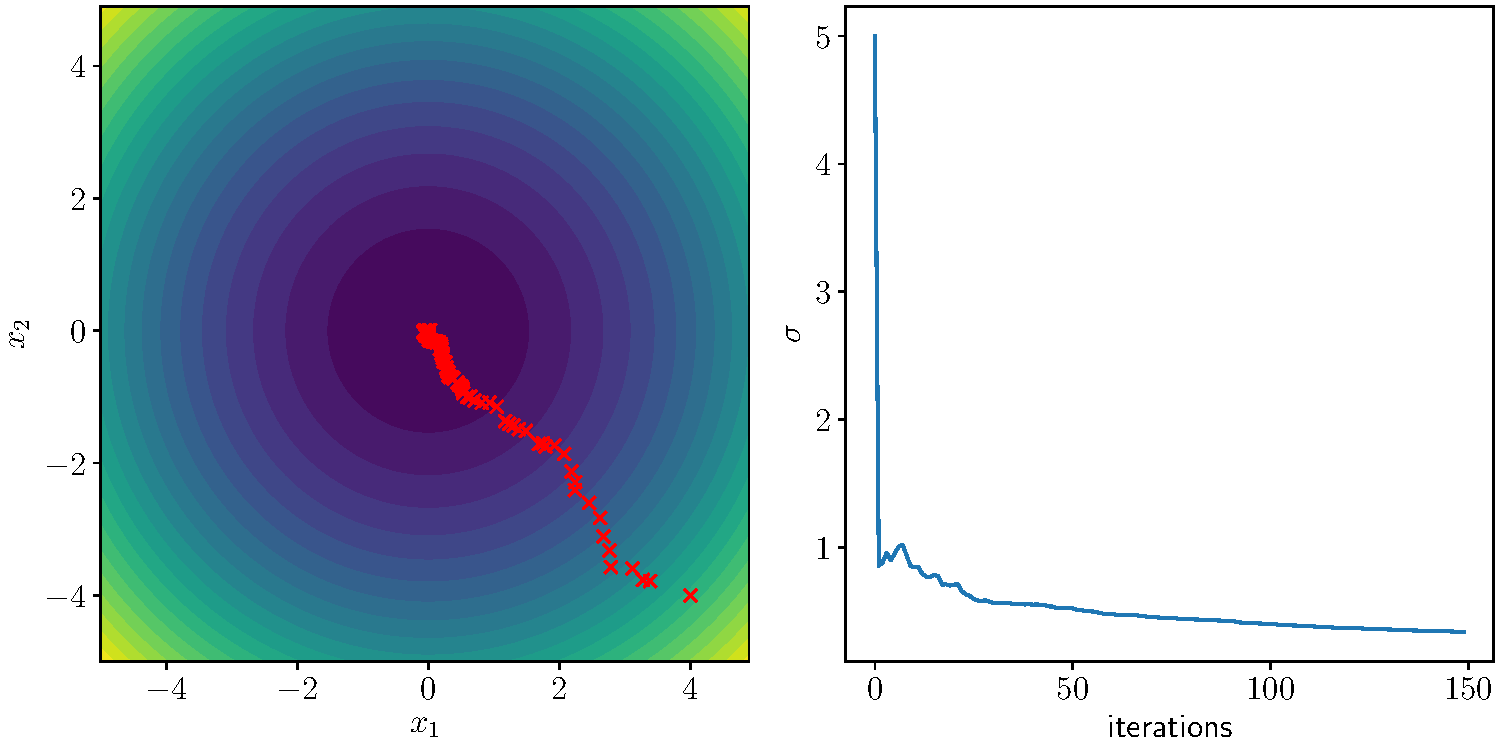
\includegraphics[width=\linewidth]{../figures/TUM/theta_evolution_VO_2023_02_21-03_34_28_PM.pdf}
		\caption{}
		\label{fig:VO_no_cons}
	\end{subfigure}
	\begin{subfigure}{0.75\textwidth}
		\centering
		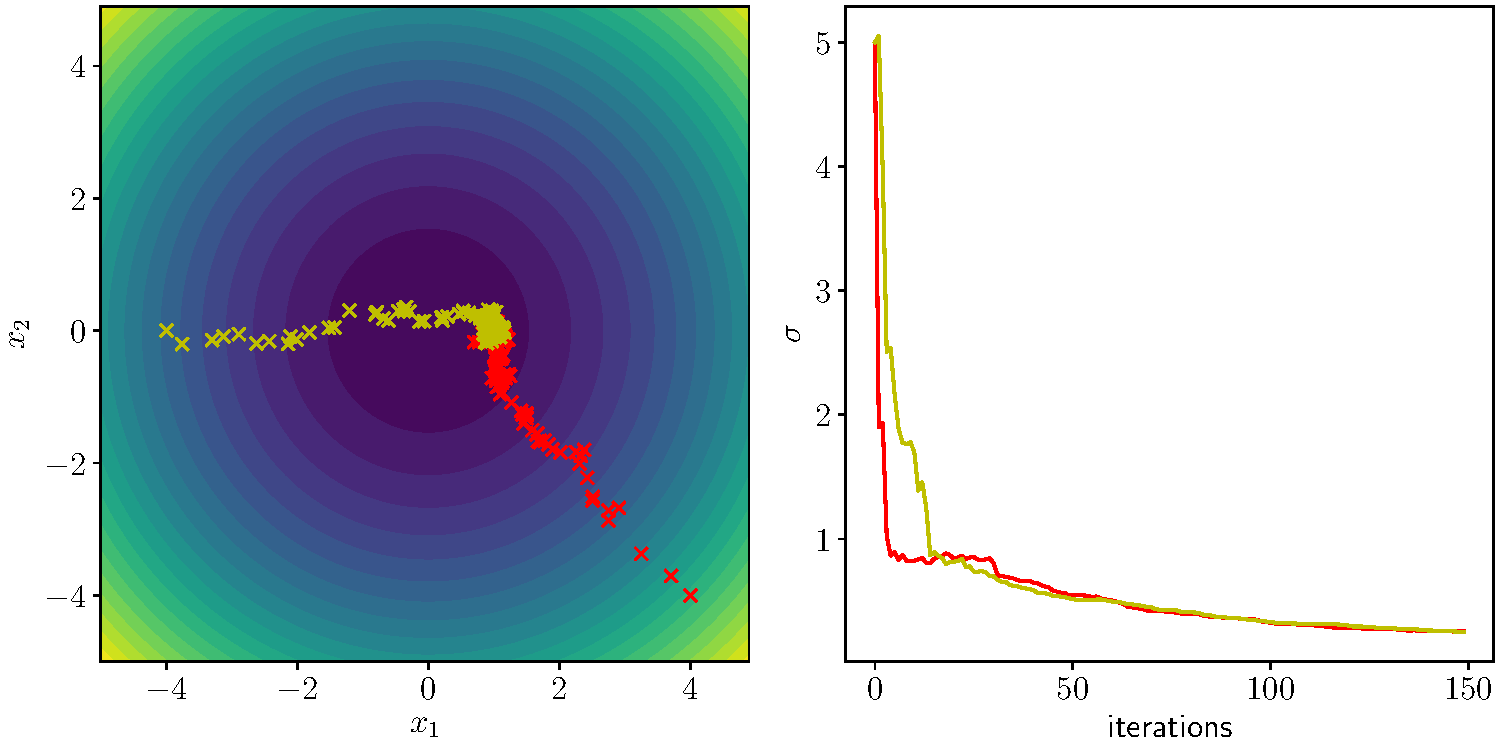
\includegraphics[width=\linewidth]{../figures/TUM/theta_evolution_VO_constraints_2023_02_24-05_12_07_PM.pdf}
		\caption{}
		\label{fig:VO_constraints}
	\end{subfigure}
	\caption{\emph{Stochastic VO for constrained and unconstrained quadratic function}: (a) This is for case when constraints are not present. The left plot shows how the Gaussian mean $\mu$ move towards the minimum of objective despite noisy gradients, the right plots the learned $\sigma$ values versus the gradient descent iterations (b) This is for a constraint on $\bm{x} (x_1 \geq 1)$. The left plot shows how the Gaussian mean $\mu$ moves towards the optimum (for two different starting values) while trying to satisfy the constraint and the right plots the learned $\sigma$ values versus the gradient descent iterations   }
	\label{fig:VO}
\end{figure}

\begin{mdframed}
	\textbf{Open research question/Novelty :} 
	\begin{enumerate}
		\item Why not use finite differences to approximate gradients?: With the constraints, the augmented objective is $C^0$, so the gradients are not even defined at that point.
		\item Then why not use Bayesian Optimization? \atul{Bayesian optimization is difficult for $(dim \geq 10)$. Also constraints are "difficult" in Bayesian optimization. The VO most probably will also struggle in high dimention. Have to check. But including constraints is not that difficult. Stelios: For the current toy problem, BO may be better (because objective has no random variable). But for the problem when the objective has implicit dependance on the design variable (through a random variable), BO makes no sense. The objective would not be known}
		\item To test in high dimention, Will it make sense to test the VO with the following?:
		\begin{align}
			f(x) = \frac{1}{200}\sum_{i=1}^{100} x_i^2 \quad \text{s.t} \quad x_i\geq1
		\end{align}
		The $\bm{x}^*$ would be a unit vector.
	\end{enumerate}
\end{mdframed}


\subsubsection{Performance based concrete design}

\begin{figure}[!htpb]
	\centering
	\begin{tikzpicture}
		\node (theta) at (-1,-2) {$\theta$};
		\node (x_1) at (0,0) {$x_1$};
		\node (x_2) at (0,-2) [circle, draw, dotted] {$x_2$};
		\node (b_1) at (1,1) [circle, draw] {$\bm{b}_1$}; % can add fill=black!20
		\node (b_2) at (1,0) [circle, draw] {$\bm{b}_2$};
		\node (y_1) at (3,1) [rectangle, draw] {$y_1$};
		\node (y_2) at (3,0) [rectangle, draw] {$y_2$}; 
		\node (y_3) at (3,-1) [rectangle, draw] {$y_3$}; 
		\node (y_4) at (3,-2) [rectangle, draw] {$y_4$}; 
		\node (C_1) at (5,1) [rectangle, draw] {$\mathcal{C}_1\left(y_1(\cdot)\right)$}; 
		\node (C_2) at (5,0) [rectangle, draw] {$\mathcal{C}_2\left(y_2(\cdot)\right)$}; 
		\node (C_3) at (5,-1) [rectangle, draw] {$\mathcal{C}_3\left(y_3(\cdot)\right)$}; 
		\node (O) at (5,-2) [rectangle, draw] {$\mathcal{O}\left(y_4(\cdot)\right)$}; 
		
		\graph {
			%A [as=$\mathcal{A}$, shape = none, "$P(A)$"];
			%B [as=$B$, shape=rectangle ,"$P(B)$"];
			%C [as=$C$,fill=black!20 , "$P(C|A,B)$"];
			
			(x_1) -> {(b_1),(b_2),(y_4)};
			(b_1) -> {(y_1),(y_2),(y_3)};
			(b_2) -> {(y_1),(y_2),(y_3)};
			(y_1) -> (C_1);
			(y_2) -> (C_2);
			(y_3) -> (C_3);
			(y_4) -> (O);
			(theta) -> (x_2);
			(x_2) -> {(y_1),(y_2),(y_3),(y_4)};
			
		};
	\end{tikzpicture}
	\caption{\emph{Stochastic computational graph for the constraint optimization problem for the performance based concrete design:} The circle represents \textit{stochastic nodes}, rectangle the \textit{deterministic node} and no shape is for the \textit{input nodes} (design variables). The objective and the constraints are explicitly dependant on the design variable $x_2$ and they are not differentiable w.r.t it (Hence $x_2$ in dotted). So based on our discussions above, $x_2 \sim q(x_2\mid\theta)$. Several other deterministic nodes are present between the random variables $\bm{b}_1$,$\bm{b}_2$ and the KPIs $y_1, y_2, y_3, y_4$ but they are ignored for brevity.}
	\label{fig:stochastic graph demonstrator}
\end{figure}

% Our idea
% Couple variatioonal optimization, baslines, penalty based optimization, automatic computational graphs.
% -- Adding constraints how it will look like
% add why no aug lamgrangian paper


% -- In practive implementation with computaional graph 
% add computational graph paper () and explain the graph